\section{Results}
\label{sec:results}

\subsection{Four options: position matters, but not toward A/B}
\label{sec:fouropt}

\begin{table}[t]
    \centering
    \caption{\mmlu with four options (1{,}500 questions, 6{,}000 prompts per model). Accuracy (\%) by position of the correct answer; each model's best position is in \textbf{bold}. Spread is best minus worst position with a 95\% bootstrap interval; ``Null'' is the spread expected from noise alone under the permutation null. Flip is the share of questions whose correctness changes with option order. $p$ is Cochran's Q, Holm-corrected. Six of seven models show a spread well above the null, but their best positions differ.}
    \label{tab:mmlu_main}
    \resizebox{\textwidth}{!}{%
    \begin{tabular}{@{}lccccclccc@{}}
        \toprule
        & & \multicolumn{4}{c}{\textbf{Accuracy with key at}} & & & & \\
        \cmidrule(lr){3-6}
        \textbf{Model} & \textbf{Balanced} & \textbf{A} & \textbf{B} & \textbf{C} & \textbf{D} & \textbf{Spread} & \textbf{Null} & \textbf{Flip \%} & \textbf{$p$} \\
        \midrule
        llama3.1-8b   & 66.0 & 61.6 & 67.3 & 66.2 & {\bf 68.8} & 7.2 \ci{5.2}{9.6}  & 1.6 & 32.6 & $<$0.001 \\
        phi3-mini     & 68.0 & 66.1 & {\bf 70.7} & 70.1 & 65.1 & 5.6 \ci{4.3}{7.7}  & 1.5 & 27.7 & $<$0.001 \\
        qwen2.5-1.5b  & 56.1 & 55.9 & {\bf 56.7} & 55.3 & 56.3 & 1.4 \ci{0.7}{3.9}  & 1.7 & 38.1 & 1.000 \\
        qwen2.5-7b    & 69.2 & 67.7 & 71.3 & {\bf 72.1} & 65.5 & 6.7 \ci{5.1}{8.5}  & 1.4 & 25.9 & $<$0.001 \\
        qwen2.5-14b   & 76.0 & 73.7 & 77.3 & {\bf 78.0} & 74.9 & 4.3 \ci{2.9}{6.1}  & 1.3 & 22.5 & $<$0.001 \\
        qwen3-4b-inst & 68.4 & 63.7 & 67.1 & {\bf 72.0} & 70.9 & 8.3 \ci{6.4}{10.4} & 1.5 & 27.6 & $<$0.001 \\
        qwen3-8b      & 67.9 & {\bf 71.4} & 63.4 & 66.6 & 70.3 & 8.0 \ci{6.1}{10.3} & 1.6 & 32.5 & $<$0.001 \\
        \bottomrule
    \end{tabular}
    }
\end{table}


\begin{figure}[t]
    \centering
    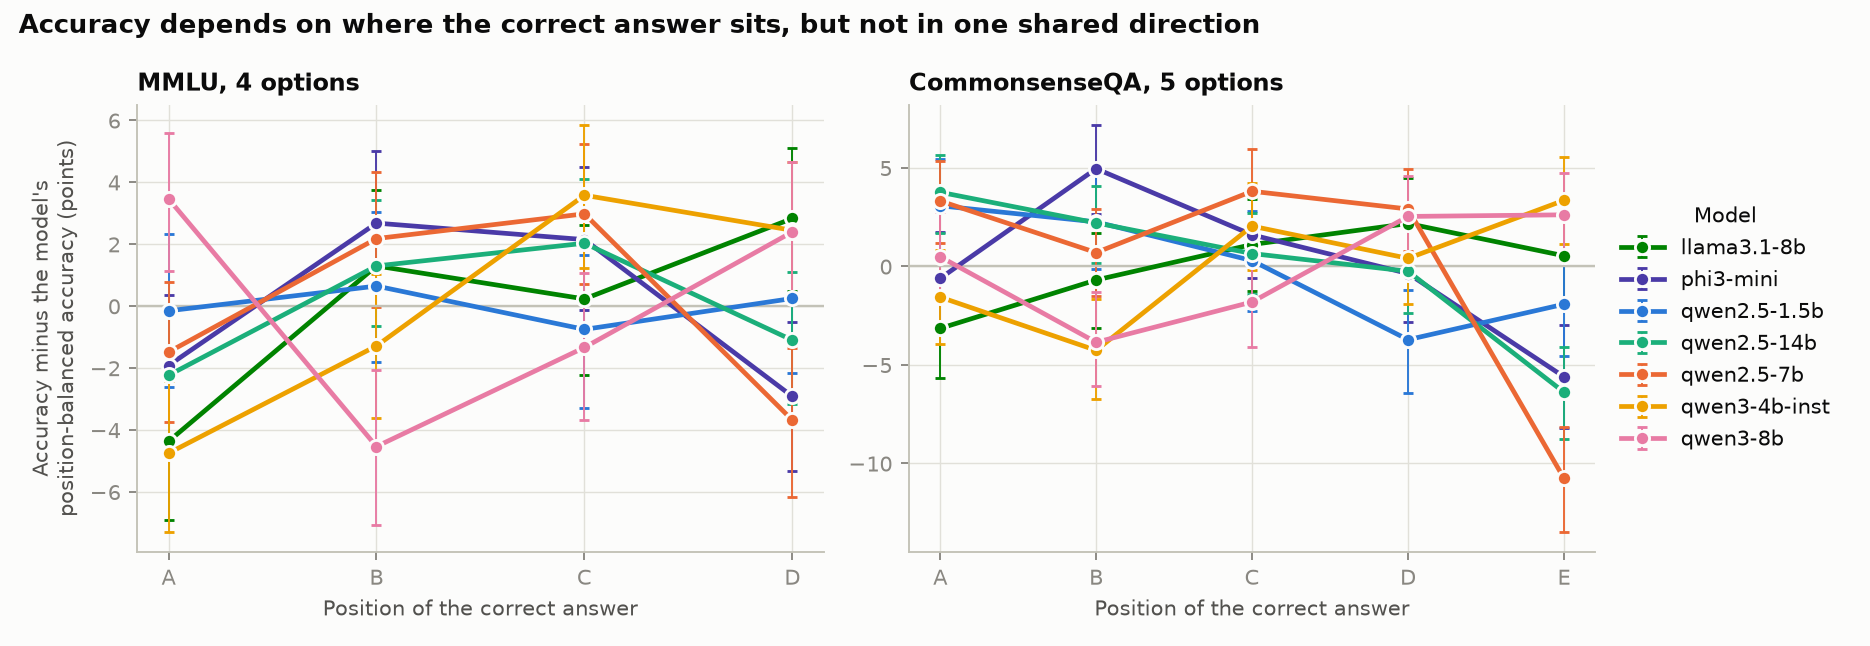
\includegraphics[width=0.95\linewidth]{figures/fig1_accuracy_by_gold_position.png}
    \caption{Accuracy by position of the correct answer, relative to each model's position-balanced accuracy, with 95\% intervals. Left: \mmlu with four options. Right: \csqa with five options. The curves cross: no position is good or bad for all models. On \csqa, the last slot (E) is the worst position for four models and the best for the two Qwen3 models.}
    \label{fig:accpos}
\end{figure}

{\bf Does position change accuracy?}
Yes, for six of seven models.
\Tabref{tab:mmlu_main} shows that the spread on \mmlu is 4.3--8.3 points for these six, against 1.3--1.7 points expected from noise alone, and Cochran's Q rejects position-independence for each of them after Holm correction.
The exception is qwen2.5-1.5b, whose spread of 1.4 is at the noise level.

{\bf Is the effect a preference for A/B?}
No.
Accuracy with the key at A is \emph{below} balanced accuracy, with the interval excluding zero, for five models, and above it for one (qwen3-8b; but see \secref{sec:robust}).
Averaged over A and B, no model gains and two lose (llama3.1-8b $-$1.5, qwen3-4b-inst $-$3.0).
Among the six models with an effect, B or C is the best position for four, D for one, and A for one (\figref{fig:accpos}).

Selection shares tell the same story (\figref{fig:share}).
With a balanced key, llama3.1-8b picks A 21.7\% of the time and D 27.1\%; qwen3-4b-inst picks A 21.5\% and D 27.3\%; qwen3-8b picks A 29.1\%.
Two models (qwen2.5-1.5b, qwen2.5-14b) are not distinguishable from uniform.

{\bf Are these patterns noise?}
No.
In a post hoc split-half check, each model's pattern replicates across two random halves of the questions: the correlation of the four position accuracies is 0.85--0.98 for the six models with a significant effect.
The patterns are stable traits of each model.

\begin{figure}[t]
    \centering
    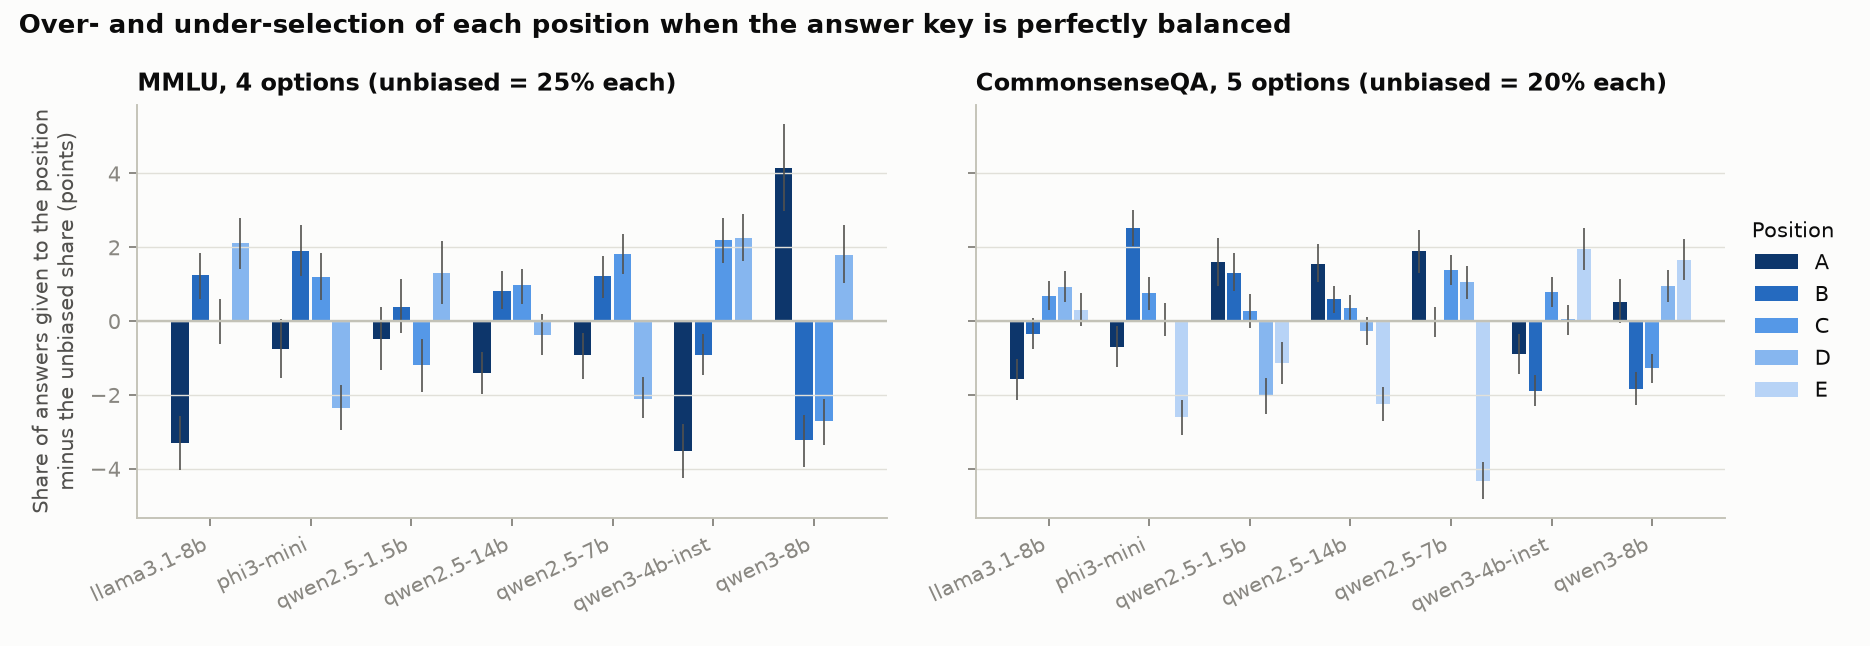
\includegraphics[width=0.95\linewidth]{figures/fig2_selection_share.png}
    \caption{How often each position is chosen, minus the unbiased share, when the answer key is balanced. Bars show 95\% intervals. Models over- and under-select different positions; several under-select A on \mmlu.}
    \label{fig:share}
\end{figure}

\subsection{How much do scores inflate?}
\label{sec:inflation}

\begin{table}[t]
    \centering
    \caption{Three definitions of inflation: accuracy minus position-balanced accuracy, in points, with 95\% bootstrap intervals. Only the best-position definition reaches the low end of the hypothesized 3--8 range, and it is biased upward because the best position is chosen after the fact.}
    \label{tab:inflation}
    \small
    \begin{tabular}{@{}llccc@{}}
        \toprule
        \textbf{Dataset} & \textbf{Model} & \textbf{As published} & \textbf{Key at A or B} & \textbf{Key at best position} \\
        \midrule
        \multirow{8}{*}{\shortstack[l]{\mmlu\\$k{=}4$}}
        & llama3.1-8b   & 0.7 \ci{$-$0.7}{2.0} & $-$1.5 \ci{$-$2.3}{$-$0.8} & 2.8 \ci{1.7}{4.2} \\
        & phi3-mini     & 1.9 \ci{0.7}{3.1}    & 0.4 \ci{$-$0.4}{1.2}       & 2.7 \ci{2.0}{4.0} \\
        & qwen2.5-1.5b  & 2.0 \ci{0.5}{3.5}    & 0.2 \ci{$-$0.6}{1.1}       & 0.6 \ci{0.3}{2.2} \\
        & qwen2.5-7b    & 1.5 \ci{0.4}{2.8}    & 0.3 \ci{$-$0.4}{1.0}       & 3.0 \ci{2.2}{4.1} \\
        & qwen2.5-14b   & 1.2 \ci{0.0}{2.3}    & $-$0.5 \ci{$-$1.1}{0.2}    & 2.0 \ci{1.3}{3.0} \\
        & qwen3-4b-inst & 0.8 \ci{$-$0.3}{2.1} & $-$3.0 \ci{$-$3.8}{$-$2.3} & 3.6 \ci{2.7}{4.7} \\
        & qwen3-8b      & 1.2 \ci{$-$0.1}{2.5} & $-$0.5 \ci{$-$1.3}{0.3}    & 3.5 \ci{2.5}{5.0} \\
        & {\bf Mean of models} & {\bf 1.3} \ci{0.7}{2.0} & {\bf $-$0.7} \ci{$-$1.0}{$-$0.3} & {\bf 2.6} \ci{2.4}{3.2} \\
        \midrule
        \multirow{8}{*}{\shortstack[l]{\csqashort\\$k{=}5$}}
        & llama3.1-8b   & $-$0.2 \ci{$-$1.4}{1.0} & $-$1.9 \ci{$-$2.8}{$-$1.0} & 2.2 \ci{1.3}{3.4} \\
        & phi3-mini     & 1.0 \ci{$-$0.3}{2.2}    & 2.2 \ci{1.3}{3.1}          & 5.0 \ci{3.7}{6.3} \\
        & qwen2.5-1.5b  & 0.3 \ci{$-$1.1}{1.7}    & 2.7 \ci{1.8}{3.6}          & 3.1 \ci{2.0}{4.6} \\
        & qwen2.5-7b    & 0.6 \ci{$-$0.7}{1.9}    & 2.0 \ci{1.2}{2.8}          & 3.8 \ci{3.2}{5.0} \\
        & qwen2.5-14b   & $-$0.2 \ci{$-$1.3}{1.0} & 3.0 \ci{2.2}{3.8}          & 3.8 \ci{2.6}{5.2} \\
        & qwen3-4b-inst & 0.1 \ci{$-$1.2}{1.3}    & $-$2.9 \ci{$-$3.9}{$-$2.0} & 3.4 \ci{2.3}{4.7} \\
        & qwen3-8b      & 0.8 \ci{$-$0.4}{2.2}    & $-$1.7 \ci{$-$2.6}{$-$0.7} & 2.6 \ci{1.9}{3.9} \\
        & {\bf Mean of models} & {\bf 0.3} \ci{$-$0.3}{1.0} & {\bf 0.5} \ci{0.0}{0.9} & {\bf 3.4} \ci{3.1}{4.0} \\
        \bottomrule
    \end{tabular}
\end{table}


\Tabref{tab:inflation} and \figref{fig:inflation} report the three definitions of inflation from \secref{sec:metrics}.

\para{As published.}
\mmlu scores sit 1.3 points \ci{0.7}{2.0} above balanced accuracy on average.
\csqa scores are not distinguishable from balanced (0.3 \ci{$-$0.3}{1.0}).
Both are well short of the hypothesized 3--8 points.

\para{Key at A or B.}
If every key were at A or B, the average model would score slightly \emph{lower} on \mmlu ($-$0.7 \ci{$-$1.0}{$-$0.3}).
On \csqa four models gain 2--3 points and three lose 2--3.

\para{Key at the best position.}
Placing every key at the position a model favors is worth 2.0--3.6 points on \mmlu for the six models with an effect, and 2.2--5.0 on \csqa.
This is the only definition that reaches the low end of the hypothesized range.
It is also biased upward, because we pick the best position after the fact; noise alone gives 0.6--0.9 points.

\begin{figure}[t]
    \centering
    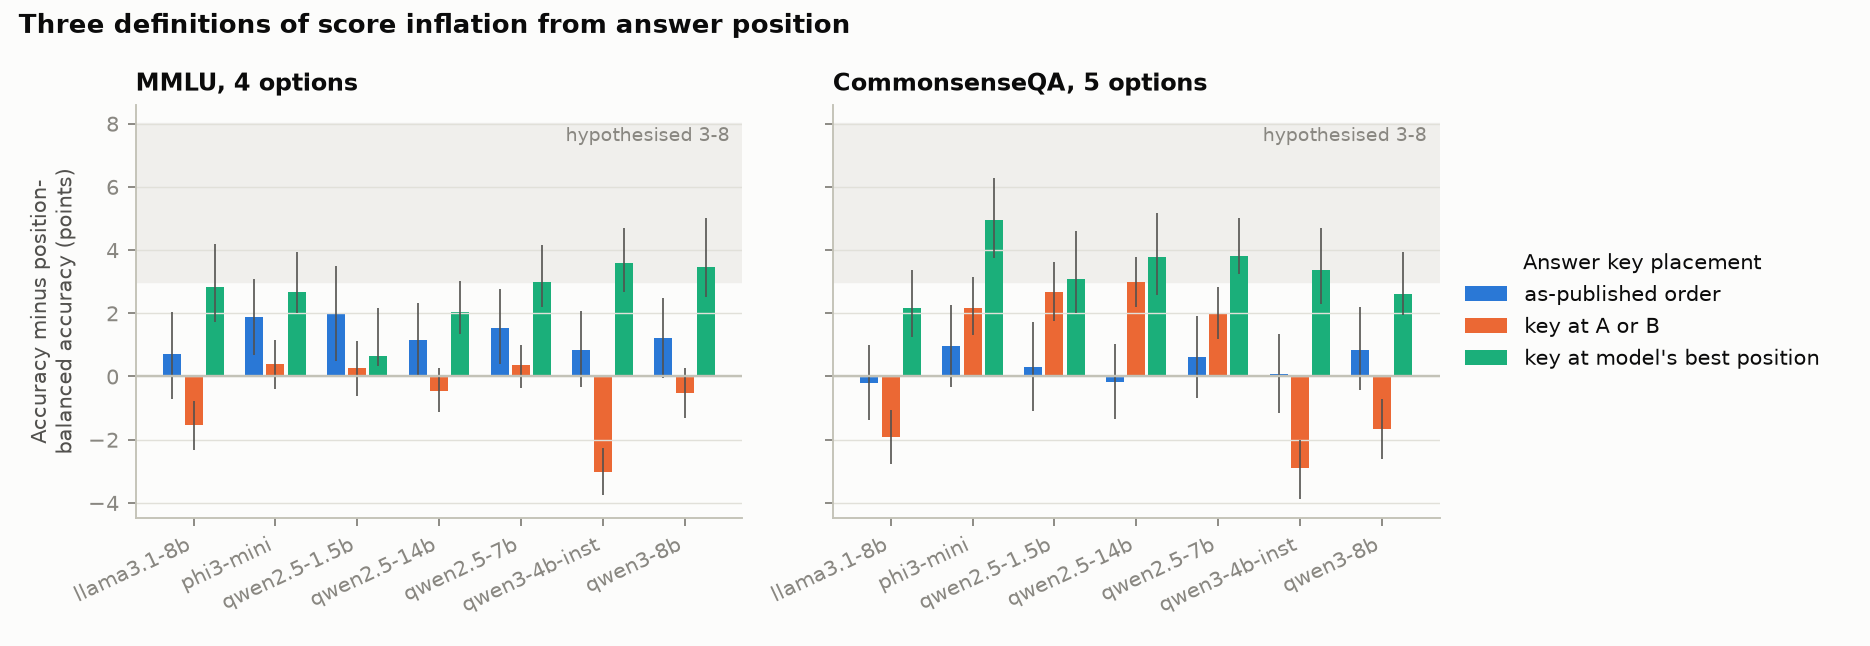
\includegraphics[width=0.95\linewidth]{figures/fig5_inflation_definitions.png}
    \caption{Three definitions of score inflation, per model, with 95\% intervals. The shaded band marks the hypothesized 3--8 points. As-published inflation (blue) stays below the band for every model, and early-key inflation (orange) is negative for several models.}
    \label{fig:inflation}
\end{figure}

{\bf Where do the 1.3 points on \mmlu come from?}
Not from key placement.
In a post hoc decomposition, we weight each model's per-position accuracy by the actual key distribution of our \mmlu sample (A 24.5\%, B 23.8\%, C 25.1\%, D 26.6\%); this predicts a gain of 0.0 \ci{0.0}{0.1}.
The whole 1.3 points therefore reflects that the published arrangement is easier than a rotation with the key in the same slot.
Part of this comes from options that only make sense in their original place, such as ``All of the above'' or ``Both A and B''.
On the 108 questions that a regular expression flags as order-dependent, the as-published advantage is 4.7 \ci{2.4}{7.5} points, against 1.1 \ci{0.5}{1.7} on the other 1{,}392.
The remaining 1.1 points is consistent with models having seen these items in their original order during training, but we cannot separate that explanation from order-dependent options that the regular expression missed.

\subsection{Option count and format}
\label{sec:format}

\begin{table}[t]
    \centering
    \caption{Position effects by format, mean of models with 95\% intervals. Spread is best minus worst position; for two options the best-position gain is half the spread. The two largest spreads (in \textbf{bold}) come from word-answer true/false and from numeric labels, not from the format with the most options. The numeric-label row excludes phi3-mini (\secref{sec:labels}).}
    \label{tab:format}
    \small
    \begin{tabular}{@{}lccccc@{}}
        \toprule
        \textbf{Condition} & \textbf{Models} & \textbf{Balanced acc.} & \textbf{Spread} & \textbf{Best-position gain} & \textbf{Flip \%} \\
        \midrule
        \boolq, True/False words & 7 & 79.5 & {\bf 14.2} \ci{13.5}{15.0} & 7.1 \ci{6.8}{7.5} & 14.6 \\
        \boolq, A/B letters      & 7 & 82.3 & 4.4 \ci{4.1}{4.9}   & 2.2 \ci{2.0}{2.5} & 6.2 \\
        \midrule
        \mmlu $k{=}2$ & 7 & 81.0 & 6.0 \ci{5.2}{6.8} & 3.0 \ci{2.6}{3.4} & 17.9 \\
        \mmlu $k{=}3$ & 7 & 72.2 & 5.7 \ci{5.0}{6.6} & 2.9 \ci{2.4}{3.3} & 24.6 \\
        \mmlu $k{=}4$ & 7 & 67.4 & 5.9 \ci{5.4}{6.9} & 2.6 \ci{2.4}{3.2} & 29.5 \\
        \mmlu $k{=}4$, labels 1--4 & 6 & 64.7 & {\bf 13.6} \ci{12.6}{14.8} & 6.2 \ci{5.7}{6.8} & 37.7 \\
        \midrule
        \csqashort $k{=}2$ & 7 & 91.8 & 2.9 \ci{2.6}{3.7} & 1.5 \ci{1.3}{1.8} & 8.4 \\
        \csqashort $k{=}3$ & 7 & 85.6 & 4.7 \ci{4.0}{5.5} & 2.4 \ci{2.0}{2.8} & 15.4 \\
        \csqashort $k{=}4$ & 7 & 81.4 & 4.6 \ci{4.0}{5.4} & 2.4 \ci{2.1}{2.9} & 21.0 \\
        \csqashort $k{=}5$ & 7 & 77.1 & 8.8 \ci{8.0}{9.9} & 3.4 \ci{3.1}{4.0} & 27.6 \\
        \bottomrule
    \end{tabular}
\end{table}


\begin{figure}[t]
    \centering
    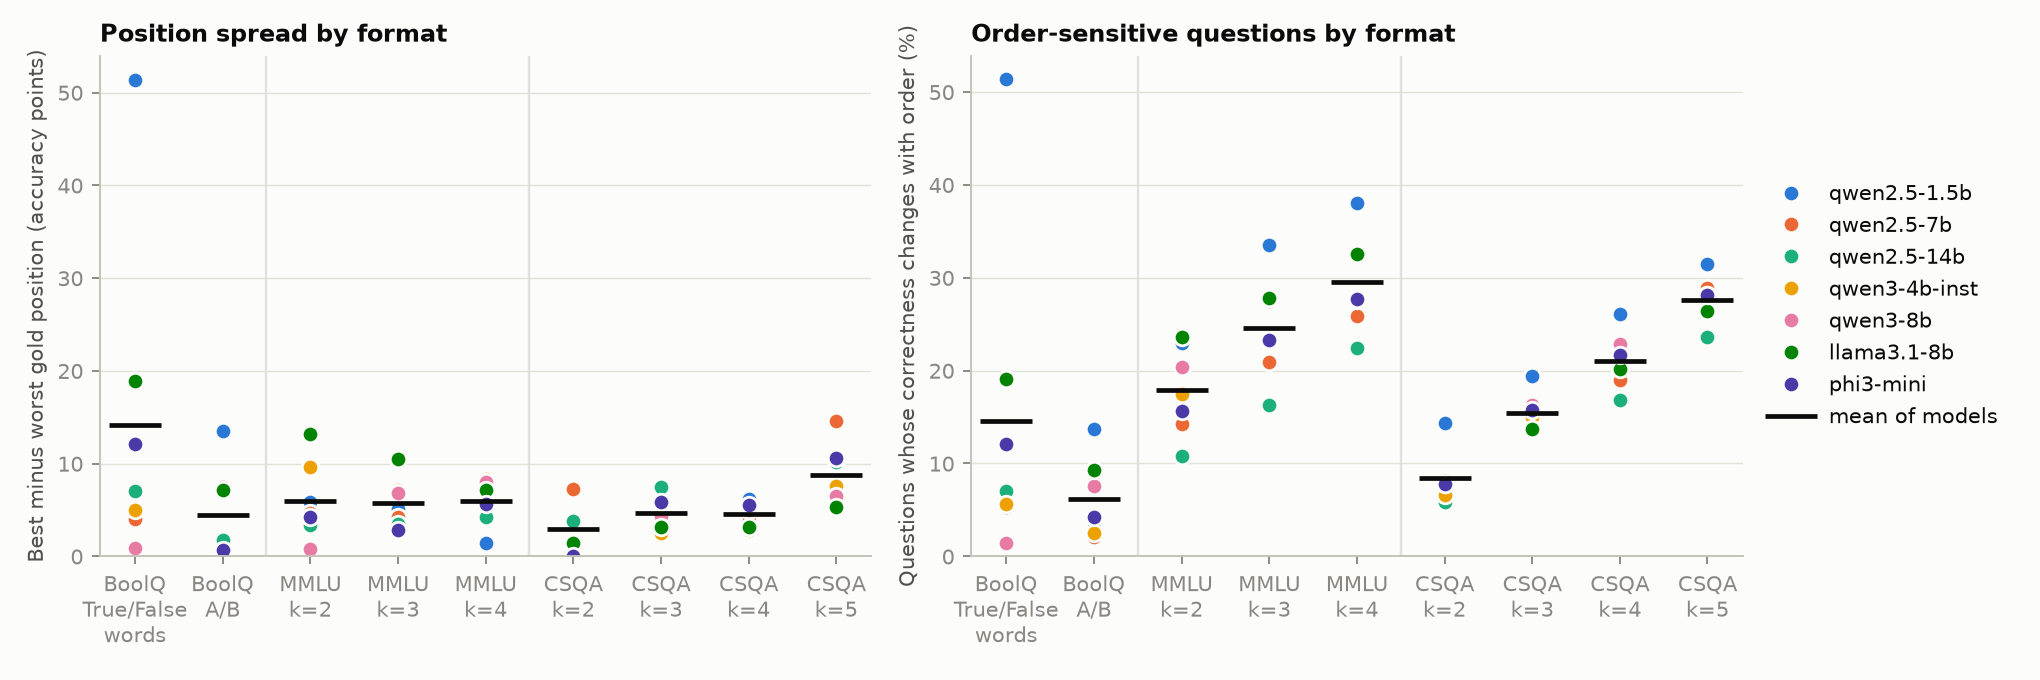
\includegraphics[width=0.95\linewidth]{figures/fig3_format_ladder.png}
    \caption{Position spread (left) and flip rate (right) by format, one dot per model; black bars are means over models. The spread is flat across option counts on \mmlu and jumps at five options on \csqa. The flip rate rises steadily with option count on both datasets. The outlier in the word-answer true/false condition is qwen2.5-1.5b.}
    \label{fig:format}
\end{figure}

\para{True/false is not the safest format.}
With word answers, the mean spread is 14.2 points, the largest in the study (\tabref{tab:format}).
The spread is under 2 points for one of seven models with word answers (qwen3-8b, 0.9) and for four of seven with A/B letters.
It is far above 2 for the rest: with word answers llama3.1-8b is at 18.9, phi3-mini at 12.1, and qwen2.5-1.5b at 51.4.
The last model picks whichever word the instruction mentions first 75.7\% of the time; it scores 90.7\% when the true answer is mentioned first and 39.3\% when it is second.
The direction again varies: four models favor the first-mentioned word and three the second.
With two options there is no averaging over positions, so a preference for one word translates directly into accuracy.

\para{Five options.}
The spread exceeds 10 points for three of seven models (qwen2.5-7b 14.6, phi3-mini 10.6, qwen2.5-14b 10.2) and averages 8.8.
On identical questions, going from four to five options raises the spread by 4.2 \ci{3.3}{4.9} points.
The increase is concentrated in one slot: four models are worse when the key is at E, three of them by 5--11 points (qwen2.5-7b drops 10.8 points below its balanced accuracy there), while both Qwen3 models are \emph{best} at E (\figref{fig:accpos}, right).

\para{Option count on its own does not drive the spread.}
On \mmlu the spread is flat from two to four options ($k{=}4$ minus $k{=}2$: 0.0 \ci{$-$0.9}{1.1}).
What rises steadily with option count on both datasets is the flip rate (\figref{fig:format}, right).
More options mean more questions whose answer changes with order, but those changes mostly cancel rather than favor a position.

\subsection{Difficulty}
\label{sec:difficulty}

\begin{table}[t]
    \centering
    \caption{Position effects by difficulty quintile, mean of models with 95\% intervals. Difficulty for a model is the mean balanced correctness of the other six models. Directed gap is accuracy at the model's overall best position minus its overall worst. The largest directed gap per dataset is in \textbf{bold}. The effect is near zero on easy questions.}
    \label{tab:difficulty}
    \resizebox{\textwidth}{!}{%
    \begin{tabular}{@{}llccccc@{}}
        \toprule
        \textbf{Dataset} & \textbf{Stratum} & \textbf{Balanced acc.} & \textbf{Directed gap} & \textbf{Flip \%} & \textbf{As-published gain} & \textbf{Position-attributable share \%} \\
        \midrule
        \multirow{5}{*}{\mmlu $k{=}4$}
        & Q1 hardest & 19.9 & 7.6 \ci{5.9}{9.5}   & 37.5 & 1.4 \ci{0.2}{2.5}       & 15.6 \ci{14.8}{21.0} \\
        & Q2         & 50.0 & {\bf 11.5} \ci{9.0}{13.8} & 55.6 & 2.7 \ci{1.3}{4.2}       & 9.1 \ci{8.3}{12.2} \\
        & Q3         & 76.3 & 6.3 \ci{4.3}{8.2}   & 34.8 & 2.5 \ci{1.3}{3.6}       & 5.8 \ci{5.1}{7.4} \\
        & Q4         & 93.1 & 3.3 \ci{2.1}{4.6}   & 14.0 & $-$0.2 \ci{$-$0.9}{0.5} & 2.2 \ci{1.8}{3.0} \\
        & Q5 easiest & 97.5 & 0.9 \ci{0.1}{1.7}   & 5.8  & 0.3 \ci{$-$0.1}{0.8}    & 0.8 \ci{0.7}{1.3} \\
        \midrule
        \multirow{5}{*}{\csqashort $k{=}5$}
        & Q1 hardest & 30.0 & {\bf 16.6} \ci{14.2}{18.8} & 49.6 & 0.0 \ci{$-$1.4}{1.7}    & 19.2 \ci{17.1}{23.1} \\
        & Q2         & 71.9 & 14.9 \ci{12.4}{17.3} & 49.4 & 1.3 \ci{$-$0.2}{2.6}    & 8.1 \ci{7.1}{10.0} \\
        & Q3         & 88.9 & 9.1 \ci{7.3}{10.9}   & 25.9 & $-$0.2 \ci{$-$1.4}{0.8} & 4.3 \ci{3.8}{5.5} \\
        & Q4         & 96.7 & 1.5 \ci{0.5}{2.5}    & 8.3  & 0.6 \ci{0.1}{1.2}       & 1.4 \ci{1.2}{2.1} \\
        & Q5 easiest & 98.1 & 1.8 \ci{1.0}{2.6}    & 4.9  & 0.0 \ci{$-$0.4}{0.5}    & 0.9 \ci{0.8}{1.4} \\
        \bottomrule
    \end{tabular}
    }
\end{table}


\begin{figure}[t]
    \centering
    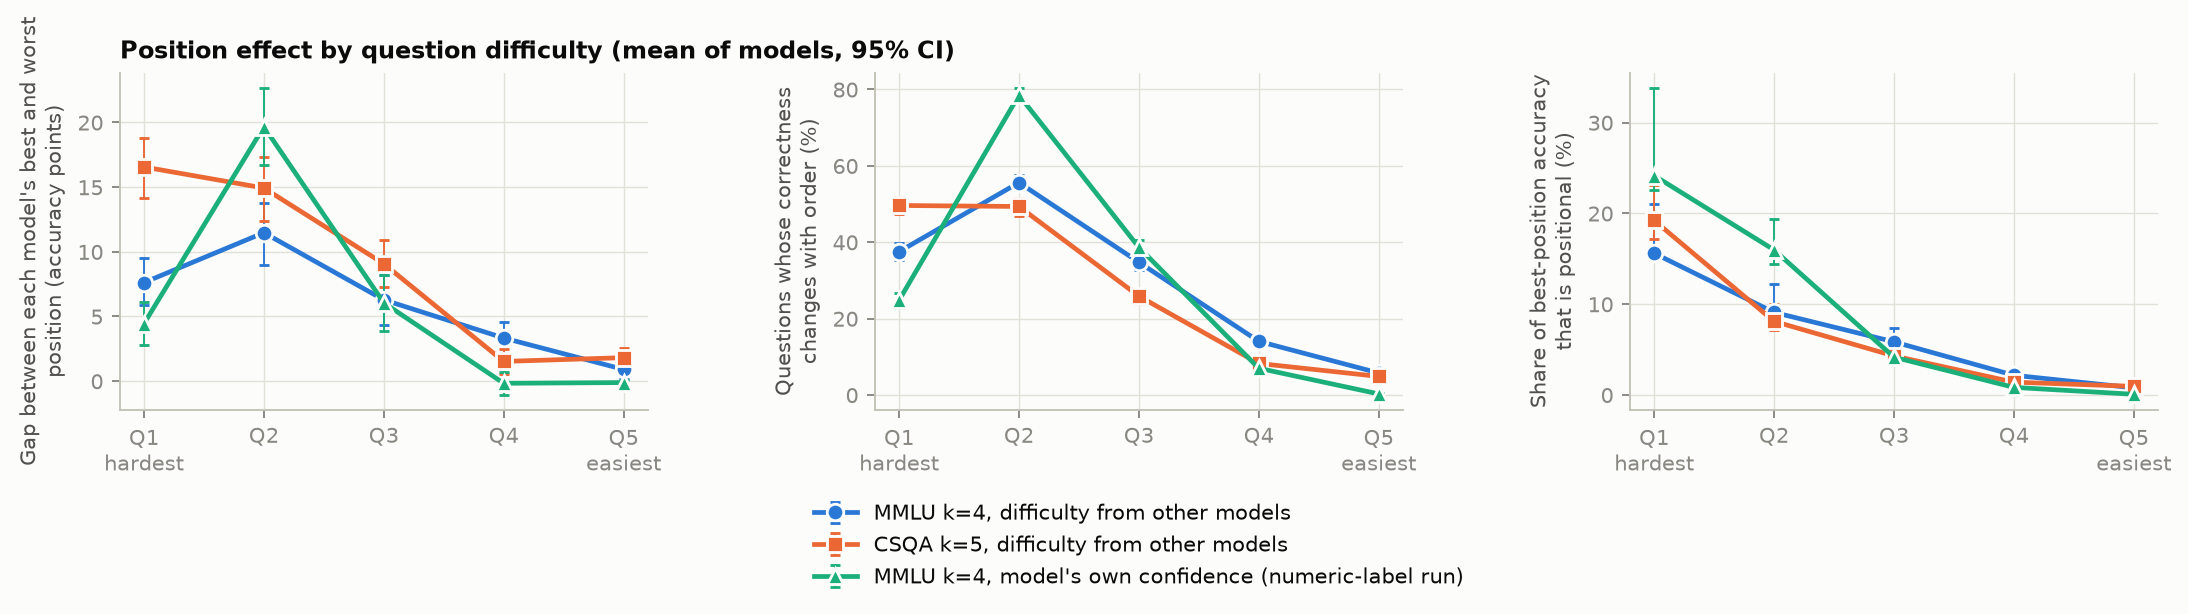
\includegraphics[width=0.95\linewidth]{figures/fig4_difficulty.png}
    \caption{Position effect by difficulty quintile, mean of models with 95\% intervals. Left: directed gap. Middle: flip rate. Right: position-attributable share. With difficulty from the other models, the gap on \mmlu peaks in the second-hardest quintile; with the model's own confidence (green) the peak is sharper.}
    \label{fig:difficulty}
\end{figure}

{\bf Is the effect strongest at medium difficulty?}
Only if ``medium'' means ``near 50\% accuracy''.
\Tabref{tab:difficulty} and \figref{fig:difficulty} show that the position effect is near zero on easy questions and large on hard ones.
When we cut questions into thirds, the middle third is \emph{not} the peak: the hard third exceeds the middle third on directed gap by 3.3 \ci{1.1}{5.7} points on \mmlu and 7.6 \ci{5.2}{9.9} on \csqa.

In quintiles, \mmlu does show a peak, at the second-hardest quintile, where balanced accuracy is 50\%.
The hardest quintile, where accuracy is 20\% and below the 25\% chance rate, has a smaller gap.
On \csqa the two hardest quintiles (30\% and 72\% accuracy) are level.

Each model's own confidence, taken from the separate numeric-label run, gives a sharper version of the same shape on \mmlu.
The gap is 19.7 \ci{16.7}{22.7} points in the quintile where accuracy is 47\%, and 78.5\% of those questions change correctness with order.
It is 4.4 points where accuracy is 8\%, and zero where accuracy is 97\% or more.
The effect therefore tracks uncertainty: it is largest where the model is close to a coin flip between a right and a wrong answer.
On these benchmarks that region is the hard-to-middle part, not the middle.

{\bf What share of accuracy is positional?}
In the hardest quintile, 15.6\% (\mmlu) and 19.2\% (\csqa) of best-position accuracy would disappear under a balanced key; in the hardest third the figures are 13.0\% and 13.4\%.
Single models go higher (qwen2.5-14b on the hardest \csqa quintile: 28\%).
These are best-case figures with the upward bias noted in \secref{sec:inflation}, and the ratios in the hardest strata have small denominators.
Measured on the benchmarks as published, the share is 6.9\% \ci{3.5}{10.1} in the hardest \mmlu third and indistinguishable from zero on \csqa.

\subsection{Label ablation: 1--4 instead of A--D}
\label{sec:labels}

\begin{table}[t]
    \centering
    \caption{Label ablation on \mmlu $k{=}4$: same questions and option order, labels A--D versus 1--4. ``First slot'' is accuracy with the key in the first slot minus balanced accuracy. The larger spread per model is in \textbf{bold}. With numerals, all six models are below balanced accuracy when the key is in the first slot.}
    \label{tab:labels}
    \small
    \begin{tabular}{@{}lcccc@{}}
        \toprule
        & \multicolumn{2}{c}{\textbf{Spread}} & \multicolumn{2}{c}{\textbf{First slot}} \\
        \cmidrule(lr){2-3}\cmidrule(lr){4-5}
        \textbf{Model} & \textbf{A--D} & \textbf{1--4} & \textbf{A--D} & \textbf{1--4} \\
        \midrule
        llama3.1-8b   & 7.2 & {\bf 22.8} & $-$4.4 & $-$14.2 \\
        qwen2.5-1.5b  & 1.4 & {\bf 10.1} & $-$0.1 & $-$3.7 \\
        qwen2.5-7b    & 6.7 & {\bf 7.1}  & $-$1.5 & $-$0.7 \\
        qwen2.5-14b   & 4.3 & {\bf 11.5} & $-$2.2 & $-$6.8 \\
        qwen3-4b-inst & 8.3 & {\bf 15.6} & $-$4.8 & $-$8.9 \\
        qwen3-8b      & 8.0 & {\bf 14.7} & $+$3.5 & $-$7.9 \\
        \bottomrule
    \end{tabular}
\end{table}


We rerun \mmlu $k{=}4$ with the same questions in the same order but with numeric labels.
We exclude phi3-mini from this comparison: it emits a whitespace token before a digit, so the first-token read-out carries no information.
Over the remaining six models, the mean spread rises by 7.7 points \ci{6.4}{8.5}, to 13.6 (\tabref{tab:labels}).
With numerals, all six models are below balanced accuracy when the key is in the first slot; llama3.1-8b scores 48.0\% there against 70.8\% in the second slot.
The size of the order effect thus depends heavily on which symbols label the options.
This fits the token-preference account of \citet{zheng2024selectors} better than a pure position account, although our design does not separate the two further.

\subsection{Does the read-out match what models write?}
\label{sec:readout}

We also answer 400 \mmlu prompts per model by greedy generation.
When the generated text contains a letter, it agrees with the first-token read-out in 97.5--99.8\% of cases across models.
The generated text contains a letter in 95.2--100\% of cases for six models and in 89.0\% for qwen3-8b, which sometimes starts an explanation instead (\tabref{tab:readout} in the appendix).

\subsection{Robustness}
\label{sec:robust}

\para{qwen3-8b is unreliable in direction on \mmlu.}
This model puts less than half of its first-token probability on any letter for at least one rotation of 391 of the 1{,}500 questions.
On the 1{,}109 remaining questions its spread is similar (7.2 versus 8.0), but the sign at position A flips, from $+$3.5 to $-$3.3.
Its apparent preference for A in \secref{sec:fouropt} is thus produced by questions where it was not going to answer with a letter.
For the other six models, the spread, the as-published gain, and the position-A effect each change by under 1 point under the same filter.

\para{Batch-composition noise.}
Rerunning qwen2.5-1.5b on 3{,}000 prompts with different batching reproduces 99.1\% of predictions; label log-probabilities move by 0.11 on average.
This comes from bfloat16 arithmetic with padded batches.
It adds up to about a point to flip rates and is unrelated to position.

\para{Multiple comparisons.}
Cochran's Q is significant after Holm correction in 57 of 70 model-by-condition cells, including 6 of 7 on \mmlu $k{=}4$ and 7 of 7 on \csqa $k{=}5$.
